\documentclass[letterpaper,12pt]{article}
\usepackage{tabularx} % extra features for tabular environment
\usepackage{amsmath}  % improve math presentation
\usepackage{float}
\usepackage{pdfpages}


\usepackage{graphicx} % takes care of graphic including machinery
\graphicspath{ {./figures/} }
%\usepackage[margin=1in,letterpaper]{geometry} % decreases margins
%\usepackage{cite} % takes care of citations
\usepackage[final]{hyperref} % adds hyper links inside the generated pdf file
\hypersetup{
	colorlinks=true,       % false: boxed links; true: colored links
	linkcolor=blue,        % color of internal links
	citecolor=blue,        % color of links to bibliography
	filecolor=magenta,     % color of file links
	urlcolor =blue         
}
\usepackage[margin = 1in,headsep=0.5cm,headheight=2cm,letterpaper]{geometry} 

\usepackage{fancyhdr}
\pagestyle{fancy}
\lhead{Student 1 : Ahmet Akman 2442366 \\ Student 2: Yusuf Toprak Yıldıran 2444149 \\ Assistant: Onur Selim Kılıç}
\rhead{Date: \today \\ Group: Wednesday Morning - 5} 
%\cfoot{center of the footer!}
\renewcommand{\headrulewidth}{0.1pt}



\begin{document}
\thispagestyle{empty}

\title{Spring 2022 EE214 Experiment 3  \protect\\ Miscellaneous Op-Amp Circuits}
\author{Ahmet Akman 2442366 \protect\\ Yusuf Toprak Yıldıran 2444149 \protect\\ Assistant: Onur Selim Kılıç}
\date{\today}
\maketitle
\tableofcontents
%\begin{abstract}
%abstract
%\end{abstract}
\section{Introduction}

\section{Experimental Results and Discussion}
The results of the experiment are discussed in the following steps.
%
\subsection{Step 1}

In first step, following circuit given in Figure X is set and it is observed that step-down operation of the tansformer under no load with sinusoidal input voltage which has a peak to peak voltage of 20 V and frequency of
50 Hz. Then, \(V_in(t) \) and \(V_out(t)\) are plotted on the graph in Figure X.

Afterwards, \(N_1:N_2\) ratio is measured as \(19.5/2.5 \approx 7.8 \).

%
\subsection{Step 2}
For this step, signal generator output is adjusted as \(𝑉_s = 10sin(2\pi50𝑡)\) with 20V peak to peak voltage and 50Hz frequency ;then, Transformer circuit with resistive load is constructed as given in the Figure X where R = \(56\Omega \).  
\subsubsection{i}

\[\]
\subsubsection{ii}
\subsubsection{iii}

%
\subsection{Step 3}
\subsubsection{i}
\subsubsection{ii}

%
\subsection{Step 4}
\subsubsection{i}
\subsubsection{ii}


\section{Conclusion}

\section*{Appendix A}
\begin{itemize}
    \item PreLab Preparation 4 hours
    \item Experimental Work 2  hours
    \item Report Writing 4 hours
\end{itemize}

\end{document}

%%%%%%%%%%%%%%%%%%%%%%   EXAMPLE TABLE   %%%%%%%%%%%%%%%%%%%%%%%%%%%%%%%%
\begin{table}[H]
\begin{center}
    \caption{Resistance reading by color code convention.}
    \vspace{2mm}
    \begin{tabular}{||c | c | c||} 
        \hline
        Color Order & Value & Tolerance \\ [0.5ex] 
        \hline\hline
        Brown / Black / Red / Gold & 1k\( \Omega \) & \( \% \) 5  \\ 
        \hline
        Yellow / Violet / Red / Gold & 4.7k\( \Omega \) & \( \% \) 5   \\
        \hline
        Brown / Grey / Orange / Gold & 18k\( \Omega \) & \( \% \) 5  \\ [1ex] 
        \hline
    \end{tabular}
\end{center}
\end{table}


%%%%%%%%%%%%%%%%%%%%%%   EXAMPLE IMAGE   %%%%%%%%%%%%%%%%%%%%%%%%%%%%%%%%
\begin{figure}[H]
\centering
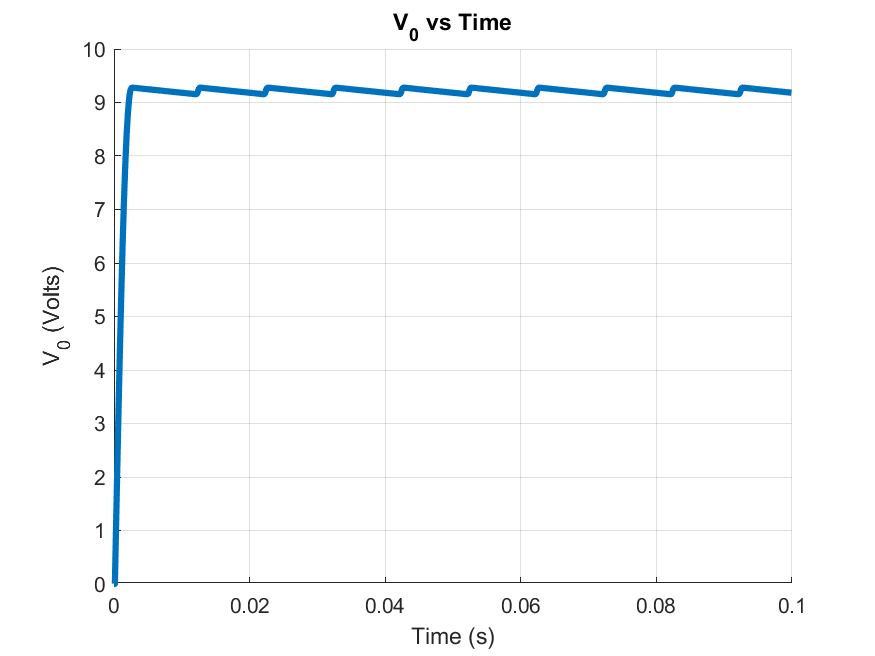
\includegraphics[width = 0.75\textwidth]{5.png}
\caption{Circuit schematic for the step 5}
\end{figure} 

%%%%%%%%%%%%%%%%%%%%%%   EXAMPLE IMAGE FROM PDF   %%%%%%%%%%%%%%%%%%%%%%%%%%%%%%%%
\begin{figure}[H] \centering{
	\includegraphics[scale=0.25]{2a_plot.pdf}}
	\caption{Experiment 2}
\end{figure}
	